\section{Simulation study}
\label{sec:al:simulations}

We utilize a simulation study in order to determine the method that is 
best-suited for usage with the VS in Chapter~\ref{ch:usage}'s financial 
application. Recall that the VS data is composed of all observations of 
characteristic features (as described in 
Section~\ref{sec:visualizer:scatterplot:features}) 
for all $n\choose 2$ pairwise scatter plots of the \textit{actual} data set 
(where $n$ is the number of variables). To 
recap, these are key features of the visualization system that 
should be (and are) captured in the simulations:

\tablespacing
\begin{itemize}
	\item \textbf{Initialization (Section 
	~\ref{sec:visualizer:al:initialization}):} 
	Initializing the active learner begins with a random selection of
	points (pairwise scatter plots) that are presented to the oracle for 
	classification. Each simulation is initialized with 10 randomly selected 
	data points.
	
	\item \textbf{Pool-based sampling (Section ~\ref{sec:al:litreview}):} After 
	initialization, $k$ unlabeled samples are randomly selected from $X$, and 
	the active learner picks one to query. Each simulation iteration (of the AL 
	algorithm) is presented $k=15$ unlabeled points to query from.
	
	\item \textbf{Random forest 
	(Section~\ref{sec:visualizer:plotgeneration:tree}):} The VS's overall 
	classification model (for use in stage 2 when stage 1 initialization and 
	querying are complete) is a random forest. Each active learning method 
	optimizes for the 
	final random forest classification model by utilizing random forests in 
	their selection process (excluding QBC due to the nature of the 
	algorithm). Instead, the QBC simulations have been run with a committee of 
	classification models that includes random forest (See 
	Section~\ref{sec:al:simulation:methods} for the full list). Furthermore, 
	the QBC simulations have been run with both (1) majority vote and (2) 
	random forest as the overarching stage 2 classification model, as well as 
	(1) with pruning and (2) without pruning.
	
	\item \textbf{Binary classification:} The classification of user 
	interests have two possible labels/levels: ``visually correlated'' (1) and 
	``not visually correlated'' (0). The simulations also use data with two 
	levels of classification (Section~\ref{sec:al:simulation:data}).
\end{itemize}
\bodyspacing

\noindent Finally, it should be noted that each active learning algorithm is 
given a budget of 50 queries (50 progressive iterations of a single trial). 
While the VS used in the financial application of Chapter~\ref{ch:usage} will 
not have such a large budget, its implementation in the simulations allows 
for proper observation of the performance of each active learning method.

\subsection{Data}
\label{sec:al:simulation:data}
The data is taken from the MNIST database of handwritten digits 
(\url{http://yann.lecun.com/exdb/mnist/}). All data have already been 
classified into digits $(0,1,...,9)$ and may be visualized in the form of a 
$28\times 28$ pixel array; the hue of each pixel is represented by a value from 
0 (light, white space) to 255 (dark, pure black). 
Each image has been transformed into a single 784-length vector by 
``unfurling'' each row and adding it to the last column of the row above it. 
For ease of use and computational efficiency, the data has been 
further compressed to a 196-length vector ($14\times 14$ pixel image). In order 
to maintain the condition of binary classification, two out of the ten digits 
were selected. The digits 7 and 9 were selected as they are visually similar, 
making it more difficult for an active learning algorithm to correctly parse 
the data with few queries (as opposed to 1 and 0, which are visually 
different). The MNIST training set contains 60,000 total data points 
while the testing set contains 10,000 total data points. For the sake of 
computational efficiency, the simulator selects 250 random samples (125 of each 
digit) from the training set to compose the final data set. 
The final data set may be visualized in Figure~\ref{fig:al:simulations:data}. 
The R functions for working with the MNIST data are adapted from file 
\texttt{gist:39760}~\cite{oconnor2008} and may be found in 
Appendix~\ref{sec:appendicies:al:simulations:data}.

\tablespacing
\begin{figure}[H]
	\begin{center}
		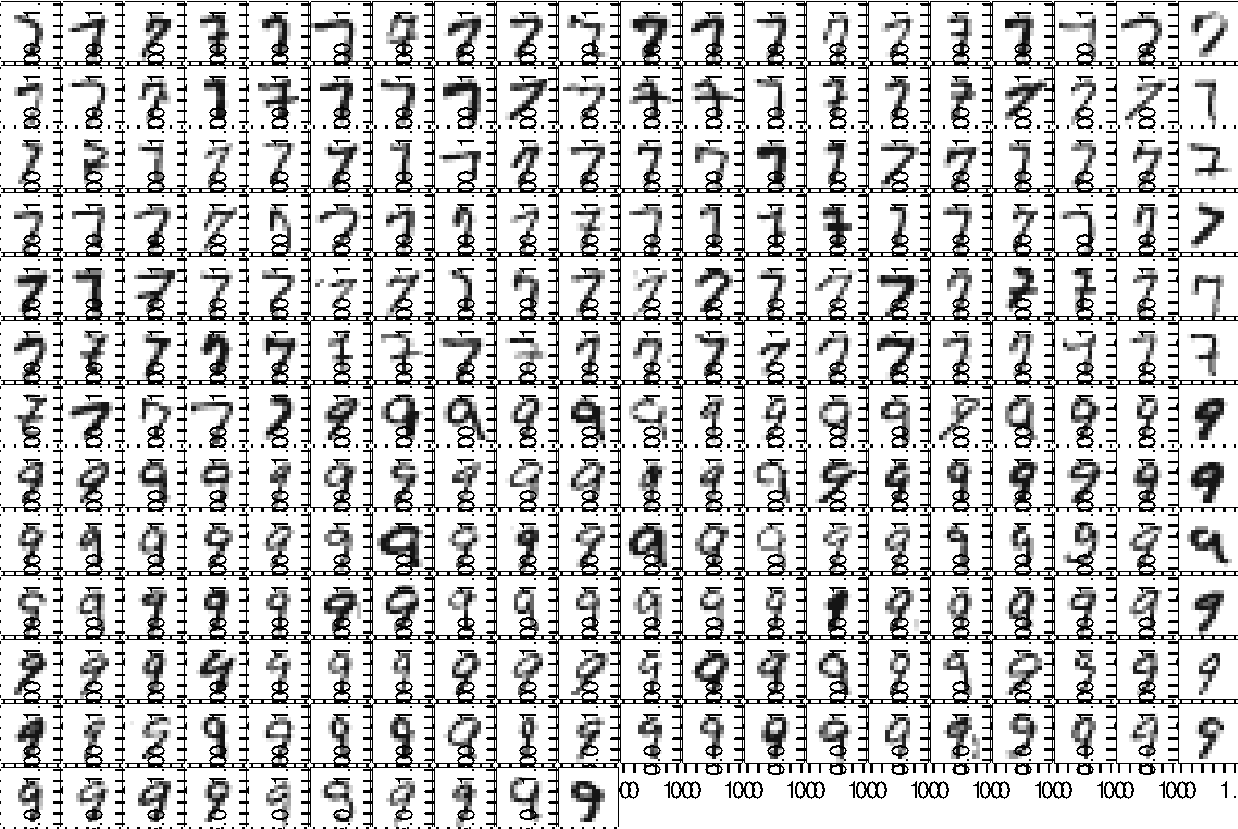
\includegraphics[width=1\linewidth]{ch-al/figures/data.pdf}
		\caption[MNIST data used in the active learning simulations.]{MNIST 
		data used in the active learning
		simulations. The digits 7 and 9 are visually similar, making 
		the simulations more realistic as it is harder for the classification 
		model to achieve a ``perfect fit'' (given only the initial labeled set) 
		without the use of querying.}
		\label{fig:al:simulations:data}
	\end{center}
\end{figure}
\bodyspacing

\subsection{Evaluation}
\label{sec:al:simulation:evaluation}
The performance of a learner at iteration (query) $j$ of trial $i$ is 
encapsulated in its error ratio $\epsilon_{i, j}$. Since there are $s=25$ 
trials 
for each active learning method, $i \in \{1,...,25\}$, and since there are 50 
iterations per trial, $j \in \{1,...,50\}$. 
Given the current labeled set, the 
\textbf{main classification model} is trained, and the entire data set is 
predicted given the resulting classifier. The predictions for iteration $j$ of 
trial $i$ are stored in an $n$-length vector $p^{i,j}$. 
We know the true labels ahead of time (thanks to the MNIST data set), and they 
are stored in an $n$-length vector $y'$. Recall that there are $n = 250$ 
variables in our data set. The predictions are compared against 
the true labels and the error ratio of iteration $j$ of trial $i$ is given by:
$$\epsilon_{i,j} = \frac{1}{n} \bigg( \sum\limits_{z=1}^{n} 
\textbf{1}_{p^{i,j}_z \neq y'_z} \bigg)$$

\noindent where $\textbf{1}_{p^{i,j}_z \neq y'_z}$ is an indicator variable 
that returns 1 if $p^{i,j}_z \neq y'_z$ and 0 otherwise. Together, these error 
ratios 
form $\epsilon$, a $25\times 50$ matrix of error ratios. Each active learning
algorithm's error ratios $\epsilon$ are averaged \textit{over each iteration} 
so that the performance of the algorithms may be compared across each 
iteration. This helps offset the randomness of the initialization and pooling 
scheme. The final, averaged error ratios are contained in a vector 
$E$ of length 50 where the average error ratio of iteration $j$ is given by:
$$E_{j} = \frac{1}{s} \bigg( \sum\limits_{i=1}^{s} \epsilon_{i,j} \bigg)$$

The final algorithm for computing $\epsilon_{i,}$, a single trial $i$'s vector 
of error ratios, is summarized as follows:

\tablespacing
\begin{algorithm}[H]
	\caption{Computing $\epsilon_{i,}$, a single trial $i$'s vector of error 
	ratios}\label{alg:al:simulation:evaluation}
	\begin{algorithmic}[1]
		\Procedure{}{$X$ is a $n\times d$ matrix of $d$ observations of all $n$ 
			variables, $y$ is an $n$-length vector of labels for each variable 
			in $X$ ($y_i$=N/A when $X_{i,}$ has no label). $y'$ is an 
			$n$-length vector of \textbf{true} labels for each variable in $X$. 
			$iter$ is the maximum number of queries allowed per trial}
		\State \textbf{loop from} $i=1$ \textbf{to} $iter$:
		\State \indent $idx \gets $ active\_learning\_method$(X,y,...)$
		\State \indent \textsc{Query} $X_{idx,}$
		\State \indent $tout \gets 
		\text{train}(X^{\text{labeled}},y^{\text{labeled}},\text{classification 
		model})$
		\State \indent $p \gets \text{predict}(tout,X)$
		\State \indent $res_i\gets \frac{\text{length}(\text{which}(p \neq y'))}
		{\text{length}(y')}$
		\State \textbf{return} $res$
		\EndProcedure
	\end{algorithmic}
\end{algorithm}
\bodyspacing

\noindent This procedure is encapsulated by 
the simulation engine code in 
Appendix~\ref{sec:appendicies:al:simulations:simengine}.

\subsection{Summary of methods}
\label{sec:al:simulation:methods}

Table~\ref{tab:al:simulations} contains a summary of the active learning 
methods used in the simulation with details such as tuning parameter values. 
As a point of comparison, random sampling is used as the control because it is 
the most simplistic base case in which active learning is not present.

\tablespacing
\begin{longtable}{p{0.15\linewidth} p{0.21\linewidth} p{0.18\linewidth} 
p{0.4\linewidth}}
	
	% First page heading
	\caption[Summary of active learning simulation methods.]{A summary of the  
	active learning methods tested in the simulation. \textit{Note:} The 
	``classification model'' column is the main classification model that is 
	used to fit the error and final classifier, not the classification 
	model(s) used in the active learning methods (which is listed under 
	\textit{classifier} or \textit{committee} in the ``parameters'' column). 
	The ``classification model'' column in the simulation is akin to the main 
	classification model in stage 2 of the VS.} 
	\label{tab:al:simulations}\\
	\toprule
	\textbf{AL method} & \textbf{Simulations} & 
	\textbf{Classification model*} & \textbf{Parameters} \\
	\midrule
	\endfirsthead
	
	% Future page heading
	\caption[]{(continued)}\\
	\toprule
	\textbf{AL method} & \textbf{Simulations} & \textbf{Main classification 
	model} & \textbf{Parameters} \\
	\midrule
	\endhead
	
	% Page footer
	\midrule
	\multicolumn{4}{r}{(Continued on next page)}\\
	\endfoot
	
	% Last page footer
	\bottomrule
	\endlastfoot
	
	Random \newline sampling \newline (CONTROL) & 
	25 trials, 50 iterations, 15 ``pooled'' points each & 
	Random forest & 
	\textit{Classifier}: None \\
	
	\cmidrule[0.1pt](l{0.5em}r{0.5em}){1-4}	
	
	Uncertainty \newline sampling ~\ref{sec:al:methods:uncertainty} & 
	25 trials, 50 iterations, 15 ``pooled'' points each & 
	Random forest & 
	\textit{Classifier}: Random forest \\

	\cmidrule[0.1pt](l{0.5em}r{0.5em}){1-4}
	
	Query by \newline committee ~\ref{sec:al:methods:qbc} & 
	25 trials, 50 iterations, 15 ``pooled'' points each & 
	Random forest &	
	\textit{Committee}: RF, NB, SVM, PLS \newline 
	\textit{Disagreement}: Vote entropy \newline 
	\textit{C\_Pruning}: T, $\epsilon$: 0.5 \\ & \\
	
	& & Majority \newline committee \newline vote &	
	\textit{Committee}: RF, NB, SVM, PLS \newline 
	\textit{Disagreement}: Vote entropy \newline 
	\textit{C\_Pruning}: T, $\epsilon$: 0.5 \\ & \\
	
	(QBC \newline CONTROL) & & Random forest &	
	\textit{Committee}: RF, NB, SVM, PLS \newline 
	\textit{Disagreement}: Vote entropy \newline 
	\textit{C\_Pruning}: F, $\epsilon$: N/A \\ & \\
	
	& & Majority \newline committee \newline vote &	
	\textit{Committee}: RF, NB, SVM, PLS \newline 
	\textit{Disagreement}: Vote entropy \newline 
	\textit{C\_Pruning}: F, $\epsilon$: N/A \\	
	
	\cmidrule[0.1pt](l{0.5em}r{0.5em}){1-4}	
	
	Query by \newline bagging ~\ref{sec:al:methods:bagging} & 
	25 trials, 50 iterations, 15 ``pooled'' points each & 
	Random forest &
	\textit{Classifier}: Random forest \newline \textit{Disagreement}: Vote 
	entropy \newline \textit{num\_class}: 5, \textit{r}: 0.75 \\
		
	\cmidrule[0.1pt](l{0.5em}r{0.5em}){1-4}	
	
	Min-max \newline clustering ~\ref{sec:al:methods:clustering} & 
	25 trials, 50 iterations, 15 ``pooled'' points each & 
	Random forest & 
	\textit{Classifier}: None \newline \textit{Distance}: Euclidean \\
	
\end{longtable}
\bodyspacing

\noindent QBC was tested with different parameters for the overall/main 
classification model (random forest vs majority committee vote) and committee 
pruning (yes or no). This was done in order to see the effectiveness of the 
addendums proposed in Section~\ref{sec:al:methods:qbc} 
(Algorithm~\ref{alg:al:methods:qbc2}) and, 
ultimately, select the best QBC method in terms of \textit{algorithm structure} 
for comparison with the other methods. Naturally, the control for comparing the 
QBC methods is the method with a random forest classification model and no 
committee pruning (this turns into the QBC methodology as detailed in 
Algorithm~\ref{alg:al:methods:qbc1}). An initial committee was selected from 
classification models that worked with the data. 
For example, consider discriminant analysis, which utilizes matrix inversion. 
The nature of the MNIST data is that many columns are 0 (white space). This is 
evident from the plots in Figure~\ref{fig:al:simulations:data}. These columns 
of 0 makes the matrix degenerate, so discriminant analysis cannot function 
without some form of data cleaning. 
To avoid further tampering with the data set (as the data has already been 
compressed), LDA, DDA, FDA, etc. were not included in the initial committee. 
A brief overview of each classification model used in the initial committee 
for QBC implementation is as follows:

\tablespacing
\begin{itemize}
	\item \textbf{Random forest:} A random forest is a collection of decision 
	trees which are grown from independent draws of the training set. A more 
	detailed description can be found in 
	Section~\ref{sec:visualizer:plotgeneration:tree}.
	
	\item \textbf{Naive Bayes~\cite{chai2004}:} 
	The naive Bayes classification model applies 
	Bayes' rule $P(y|x) = \frac{P(x|y)P(y)}{P(x)}$ to compute the posterior 
	probability $P(y|x)$ of sample $x$ belonging to label $y$ and uses the 
	results to classify the data. It is important to note that the algorithm 
	assumes independence among the features that characterize each label, which 
	may not necessarily be the case.
	
	\item \textbf{Support vector machine~\cite{tong2001}:} 
	In the support vector machine classification model, the data in $X$ is 
	mapped to a space in $\mathbb{R}^2$, which is split by a hyperplane that 
	separates the data as much as possible. Data is labeled according to its 
	side. As an active learner, the SVM queries from the point closest 
	to the linear decision boundary. SVMs can also perform nonbinary and 
	nonlinear classification through the usage of a kernel.
	
	\item \textbf{Partial least squares~\cite{boulesteix2006}:} 
	In partial least squares, 
	a \textit{principle component analysis} is first performed on the data set 
	$X$. Principle component analysis 
	takes the $n$-length set of variables in $X$ (which may or may not be 
	correlated) and converts them into some set $X'$ of linearly uncorrelated 
	``principle components''. Principle components are not necessarily 
	individual variables; they may instead be a combination of variables (e.g. 
	$X_iX_j$, $X^2_iX_j$, etc.), thereby accounting for potential dependence in 
	the data. PLS then selects the principle components which best explain the 
	observed response in $Y$ (the labels), performs a linear regression on the 
	selected components, and uses the results in order to classify the data. 
\end{itemize}
\bodyspacing

The call to each active learning function is controlled by the active learning 
engine code found in Appendix~\ref{sec:appendicies:al:simulations:alengine}. By 
implementing the active learning call in this way, the main active learning 
functions are hidden from the end user so that they cannot call the functions 
directly, which may lead to bypassing checks and/or improperly calling 
functions.



\subsection{Results}
\label{sec:al:simulation:results}

The full simulator which loads the data (using functions in 
Appendix~\ref{sec:appendicies:al:simulations:data}), calls the simulation 
engine 25 times for each active learning method (the simulation engine, 
Appendix~\ref{sec:appendicies:al:simulations:simengine}, calls the active 
learning engine, Appendix~\ref{sec:appendicies:al:simulations:alengine}), 
and plots the averaged error ratios may be found in 
Appendix~\ref{sec:appendicies:al:simulations:results}.

\begin{figure}[htb]
	\begin{center}
		\includegraphics[width=1\linewidth,page=2]{ch-al/figures/results.pdf}
		\caption[Active learning simulation results for query by committee with 
		varying parameters.]{Active learning simulation results for query by 
			committee with varying parameters. Each of the 25 trials were 
			consistently seeded with its own value, so the values before 
			committee pruning would/would not have occurred (at $iter/2=25$) 
			are the same. }
		\label{fig:al:simulations:resultsqbc}
	\end{center}
\end{figure}

Figure~\ref{fig:al:simulations:resultsqbc} is a summarization of the 
performance of query by committee with parameters specified in 
Table~\ref{tab:al:simulations}. With the main classification model, majority 
committee vote outperforms random forest on 
average in the first half (25 iterations). What is interesting to note in 
iteration 25 onwards is that the error ratio for majority committee vote (with 
committee pruning) spikes up \textit{after pruning has occurred}. 
This is interesting since the idea was to prune committee who performed poorly; 
this indicates that the insight of \textit{all} committee members, 
despite performance (or with more room for error than $\epsilon = 0.5$), are 
valuable. 
Naturally, this phenomenon cannot be observed in the random forest (with 
committee pruning) results because the classification model is a random forest; 
since committee members are not weighing in on the final predicted labels, the 
members themselves hold less weight. Although majority committee voting 
(without committee pruning)
continues to maintain its lead past 25 iterations, the error ratios converge as 
the number of iterations gets closer to 50. In fact, near iteration 50, it 
appears that both random forest methods (with and without committee pruning) 
start converging faster and just barely overtake majority committee vote 
(without committee pruning) at the end. In other words, QBC with majority 
voting (without committee pruning) starts off better but improves more slowly 
while QBC with random forest (both with and without committee pruning)
starts off worse but improves more rapidly.
Each method has its own trade-offs, so it becomes all the more important to 
keep the end goal, the visualization system, in mind. Recall that an important 
criterion for active learning performance is performance given {less query
points}. The user should not have to label more than fifty plots in order for 
the system to learn his/her interests; not only is it tedious for the user, but 
this tedium may cause the user to perform the tasks with less seriousness or 
cause the user's concentration to slip. Subsequently, we select \textbf{QBC 
with majority committee vote and no committee pruning} for comparison with the 
other algorithm types.

\begin{figure}[htb]
	\begin{center}
		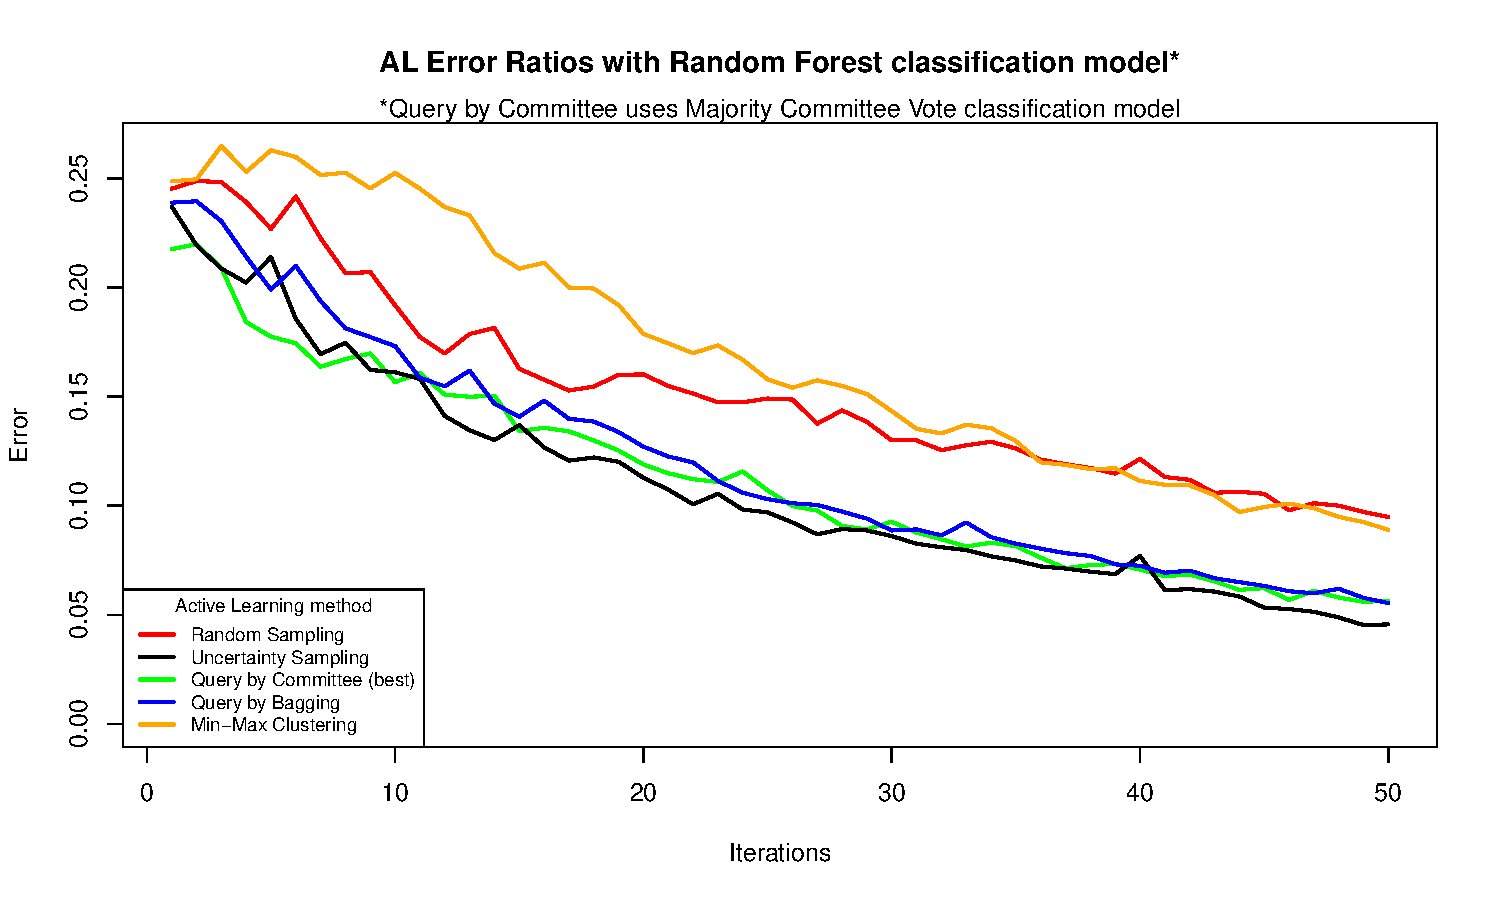
\includegraphics[width=1\linewidth,page=1]{ch-al/figures/results.pdf}
		\caption[Aggregated active learning simulation results.]{ 
		Aggregated active learning simulation results. Parameters for each 
		method may be found in Table~\ref{tab:al:simulations}.}
		\label{fig:al:simulations:results}
	\end{center}
\end{figure}

Figure~\ref{fig:al:simulations:results} summarizes the performance of the 
selected QBC method against the other active learning methods and random 
sampling as a control (a baseline for comparisons). Random sampling actually 
performs better than one might expect, though it is the first to fall off 
(converge more slowly). This may be, in part, due to the constraints of 
pool-based sampling. In each iteration, random sampling was also constrained to 
15 random points to query from. Thus, each active learning method cannot 
optimize over the entire sample space.

What is especially interesting is that random 
sampling performs better than min-max clustering for the longest time, but 
min-max clustering converges more rapidly and eventually overtakes random 
sampling. This may be attributed to the nature of the active learner's 
initialization. With clustering algorithms, initialization is extremely 
important; by starting within a cluster, the min-max methodology 
allows the learner to sample more informative labels 
without having to search through the entire space for clusters. 
In the simulator, recall that each active learning method is initialized 
randomly with the same set of data and starting points. We suspect that if we 
had initialized the min-max clustering method with the $k$-nearest neighbors 
graph as suggested by Vu \textit{et al.}~\cite{vu2010}, the min-max 
clustering algorithm would have performed better. 

Query by bagging, overall, performs worse than query by committee. In fact, it 
performs similarly to QBC with a main random forest classification model, whose 
performance can be seen in Figure~\ref{fig:al:simulations:resultsqbc}. 
This isn't surprising because the bagging algorithm itself uses a committee of 
5 random forest classifiers and also uses a random forest for the main 
classification model. 

There appears to be another ``tie'' between query by committee and uncertainty 
sampling. QBC starts off better, but the faster convergence in uncertainty 
sampling eventually outperforms QBC around iteration 10. Unlike the case of QBC 
with a random forest versus majority committee vote classification model 
(Figure~\ref{fig:al:simulations:resultsqbc}), uncertaintly sampling overtakes 
QBC much earlier. Thus, out of all methods described in 
Table~\ref{tab:al:simulations}, \textbf{uncertainty sampling} most closely 
embodies the qualities that characterize a strong active learner: intelligent 
selection of queries that allow the main classifier to learn interests more 
quickly. It would seem natural to select $iter = 10$ for the financial 
application in Chapter~\ref{ch:usage}, but recall in 
Section~\ref{sec:visualizer:al:initialization} that we would like to compensate 
for the randomness in the initialization by providing a larger query budget. As 
such, the VS stage 1 budget is set to $iter = 15$ for the financial application.

\begin{figure}[htb]
	\begin{center}
		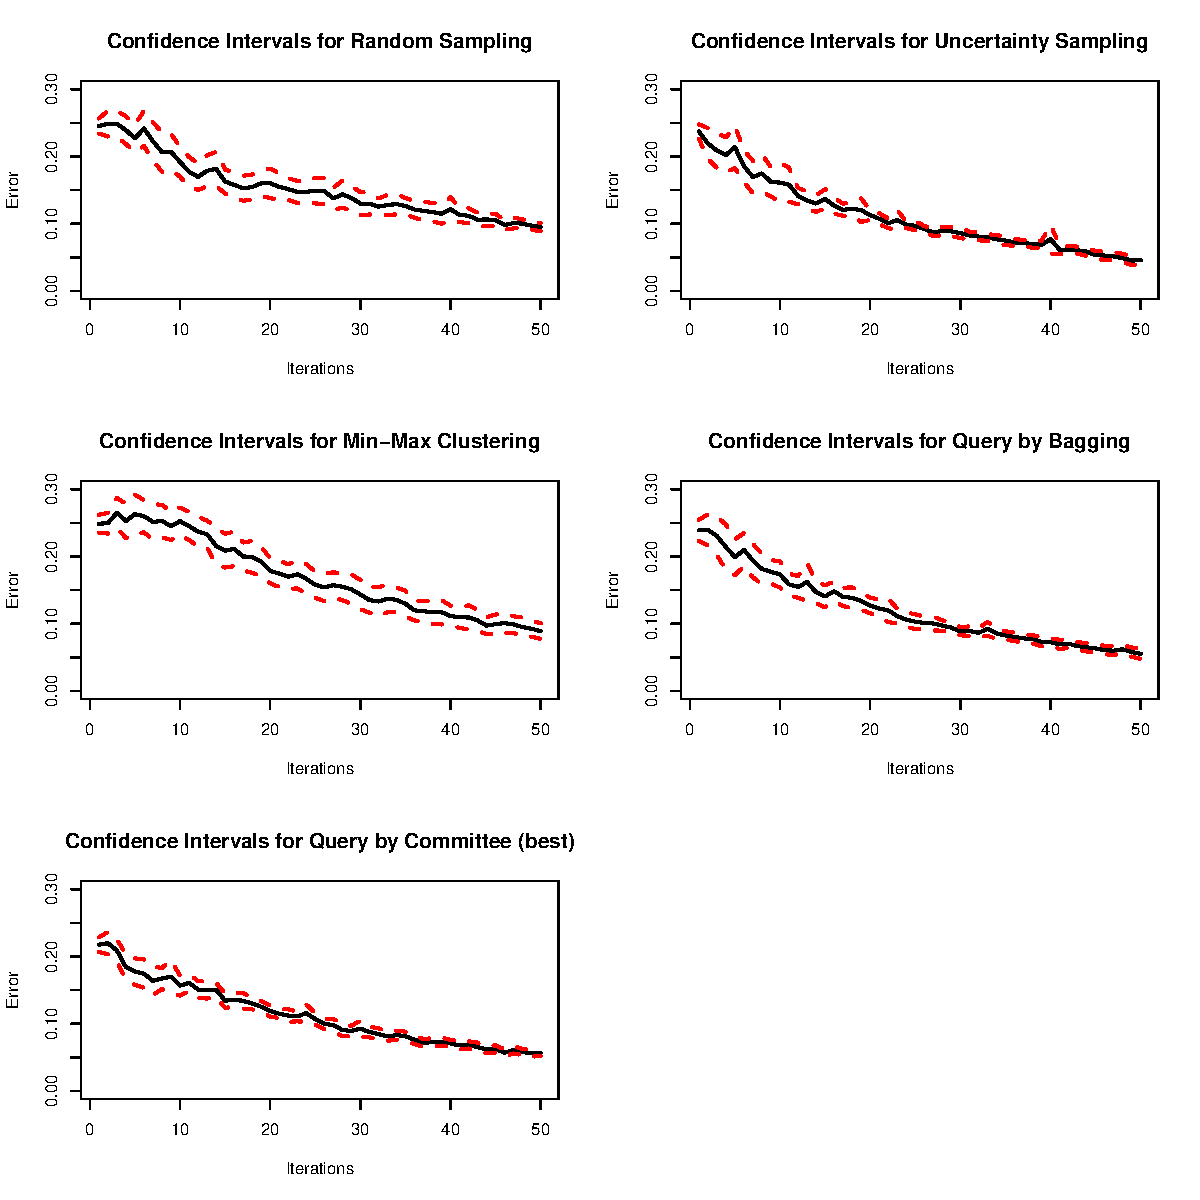
\includegraphics[width=1\linewidth]{ch-al/figures/results_ci.pdf}
		\caption[Active learning simulation results with confidence 
		intervals.]{Active learning simulation results with confidence 
		intervals.}
		\label{fig:al:simulations:resultsci}
	\end{center}
\end{figure}

Figure~\ref{fig:al:simulations:resultsci}, which plots the performance of each 
active learning method with confidence intervals, is also of interest. In 
general, as the number of queries (iterations) increases, the confidence 
interval shrinks, indicating that the data classification is less variant and 
more accurate. This is not the case for min-max clustering, however; both the 
error and the confidence interval converge more slowly, underscoring the 
importance of initialization in clustering methods. 
We may also observe that the confidence interval is rather small at iteration 
1. This may be attributed to the simulation being seeded at each trial before 
each trial's first iteration, thereby causing less variance at the start.

\subsection{Extensions}
\label{sec:al:extensions}

There are many other parameters that could have been tested but were 
not in the interest of time. For 
example, the classification model used in the active learning method to aid in 
query selection does not have to be a random forest 
(this applies to uncertainty sampling and query by bagging); perhaps another 
would have worked better despite 
the intuition that, if the active learning methods optimize over the same 
classification model that the main program (the VS, in this case) will use, the 
learner will perform better. As noted earlier, initialization is important for 
efficient min-max clustering, so the performance of the 
learner could also be tested with different initialization 
schemes. Furthermore, there are other disagreement methods 
that could be implemented aside from vote entropy, one of which was described 
earlier in Section~\ref{sec:al:methods:qbc} (this applies to query by committee 
and query by bagging). The tuning parameters of $\epsilon$ in QBC and $r$ in 
QBB could also be perturbed to see the effect on the error ratio. Perturbing 
$\epsilon$ may also provide insight into why QBC suddenly performs worse the 
moment a committee is pruned. Finally, 
different initial committees could be fed into the QBC method, and different 
starting points for committee pruning (e.g. $iter/3$ or $iter/4$ instead of 
$iter/2$) could also be tested.